\documentclass[letterpaper]{sig-alternate}


\pdfpagewidth=8.5in
\pdfpageheight=11in

%\usepackage[factor=250,spacing=true]{microtype}

\begin{document}
\conferenceinfo{RecSys '14}{October 6--10, 2014, Foster City, Silicon Valley, USA}
%\CopyrightYear{2007} % Allows default copyright year (20XX) to be over-ridden - IF NEED BE.
%\crdata{0-12345-67-8/90/01}  % Allows default copyright data (0-89791-88-6/97/05) to be over-ridden - IF NEED BE.

\title{TODO: title}

\numberofauthors{2}

\author {
\alignauthor
Daniel Kluver\\
\affaddr{GroupLens Research}\\
\affaddr{Department of Computer Science and Engineering}\\
\affaddr{University of Minnesota}\\
\affaddr{Minneapolis, MN 55455 USA}\\
\email{kluver@cs.umn.edu}
\alignauthor
Joseph A. Konstan\\
\affaddr{GroupLens Research}\\
\affaddr{Department of Computer Science and Engineering}\\
\affaddr{University of Minnesota}\\
\affaddr{Minneapolis, MN 55455 USA}\\
\email{konstan@cs.umn.edu}
}

\maketitle
\begin{abstract}

TODO: abstract

\end{abstract}

%TODO: update these things.
% A category with the (minimum) three required fields
\category{H.4}{Information Systems Applications}{Miscellaneous}
%A category including the fourth, optional field follows...
\category{D.2.8}{Software Engineering}{Metrics}[complexity measures, performance measures]

%TODO: update these things.
\terms{Theory}

%TODO: update these things.
\keywords{ACM proceedings, \LaTeX, text tagging}

\section{Introduction}
  % describe new user experience in recommender systems.
  When someone first interacts with any intelligent system, the system knows nothing about them.
TODO:
  

  % new user experience is important, and here is why.
    % talk about first impressions and user trust
  The new user experience is a very important part of any recommender system.
  The first interaction with a system is the only chance the system gets to make a first impression on the user.
  This first impression can be very important in structuring a user's expectations for how the system will behave, and determining how much the user trusts the system's recommendations.
  If the system behaves poorly when the user is new, then the user may leave and not come back.
  This is especially a concern with recommender systems which rely on large amounts of user information to make personalization decisions.
  When users are new the system will not have much information to personalize the user experience which may lead the user to leave the system.
  
  % Past work on cold start has focused on… (how long should this section be?)
    % ways to sort items to get to most value out of early ratings
    % research looking at user experience and other forms of data collection

  Past work has referred to the new user experience issue as the \emph{user cold start} problem.
  This work has normally focused on two
TODO:

  % How an algorithm behaves the first time a user sees it is important (first impression)
    % Past work looks carefully at issues X, Y, and Z, but doesn’t take a systematic look at the behavior of algorithms for users with few ratings.
  % Our work sits at the intersection of two important fields of recommender system research: New user experiance, and comparing algorithms. While there has been much work comparing various algorithms, there has been little formal work comparing algorithms based on their performance for new users. Therefore our work focuses on the behavior of recommender algorithms across different amounts of user data. (subsection might need re-ordering)
  % RQs
    % RQ1 How do the behavior of different algorithms change with the number of ratings?
      % Explain that there are a lot of different ways to measure algorithm behavior.
        % Predictive accuracy, commonly measured with MAE or RMSE
          % coverage
        % Value of recommendations, tradidionally done with metrics from information retrieval such as precision, recall, MAP, etc. These algorithms try to measure ...
          % cite the John/Joe paper (RMSE is not enough)
          % cite the paper cited by 10 is enough
          % topN RMSE
        % There are many properties of recommenders that are (find words here)
          % popularity
          % diversity
          % spread
      % RQ1A  How does algorithm behavior change with respect to predictive accuracy?
      % RQ1B  How does algorithm behavior change with respect to TopN recommender performance?
      % RQ1C How does algorithm behavior change with respect to other metrics such as popularity and diversity?


    % We look at three families of recommender algorithms (user based KNN, item based KNN, SVD)
    % we compare on several dimensions
    % we suggest a methodology for performing these types of computations



\section{Methodology}
  % (high level description/restatement of approach) To answer our research questions we will various metrics of recommenders in an offline setting simulations users as they join the system.
    % maybe hit some limitations
    % motiviate _why do a simulation_ (a lot of metrics we want to try)
  % temporal replay evaluation 
    % similar technique, harder to do than ours, and with a different goal.
  % SOMEWHERE AROUND HERE talk about drnner and adaptive bootstrapping and 10 isenough paper's ad hoc plots by datapoint size.
  % algorithms (discuss tuning of algorithms per algorithm?)
    % item mean baseline
    % user adjusted baseline (@michael, is there a cite for this?)
    % user-user
    % item-item
    % SVD
  % metrics (expected / good behavior for each metric (I.E. this should go down, any reasonable algorithm should always beet baseline)) 
    % accuracy metrics 
      % RMSE
    % recommendation performance metrics (list subject to change)
      % ndcg
      % MAP@N (not yet measured)
      % precision@N
      % fallout @ N
      % RMSE of recommended items
      % (note that we looked at MRR and recall, but found them to behave the same).
    % other properties
      % recommendation average popularity
      % recommendation diversity
      % spread (entropy of recommendations) (related to recommendation coverage)

  % dataset
    % # user
    % # items
    % distributions of # ratings per user (important: min 20)
  % subsampling strategy
    % describe normal crossfold solution
    % describe issues with solution
    % describe our crossfold then subsample solution.


\section{Results}

  Using the methodology described in \cite{sec:methodology} we compute a value for each metric on each of the five algorithms.
  We plot these results against the number of items retained.
  These plots allow us to compare the algorithms against each other, and also, to understand how each algorithm's performance changes with more data.
  Each plot will have error bars showing the 95\% confidence intervals around the average per use value for the metric.

\subsection{Prediction accuracy}
  % Prediction accuracy
\begin{figure*}
  \centering
  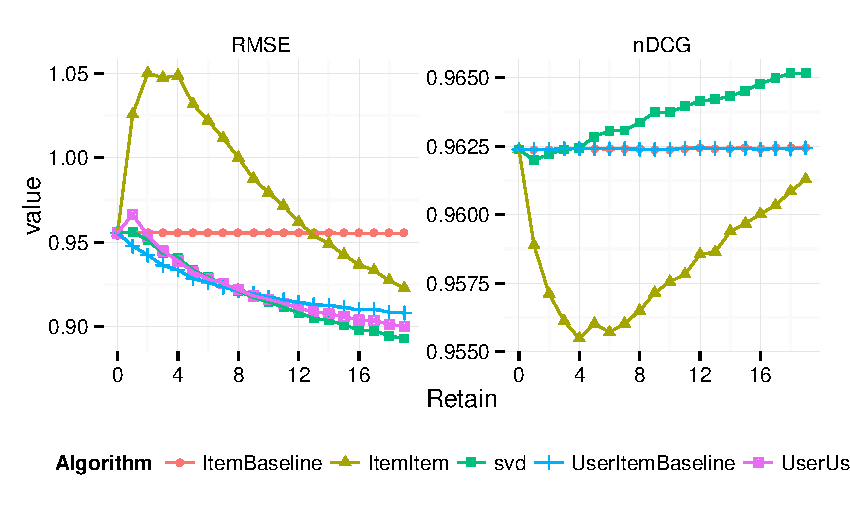
\includegraphics[width=\linewidth]{/export/scratch/kluver/workspace/coldstartrecommendation/lenskit/output/ekstrandTuning/accuracy.pdf}
  \caption{TODO}
  \label{fig:rmse}
  \label{fig:ndcg}
\end{figure*}
    % RMSE plot
    % point out error bars etc.
    % explain / interpret plot
  Figure \ref{fig:rmse} shows how accurate our algorithms are as measured by RMSE.
  As would be expected the accuracy of our item baseline doesn't change as the amount of information changes.
  The User-User and svd algorithms both perform as expected, starting out with the same accuracy as the item baseline, and then monotonically improving.
  User-User does show a small increase of error with only one rating, but the change is quite small and unlikely to be noticed by users.
  Interestingly, User-User and svd both perform about as well as our smarter user item baseline. %TODO: explain this better

      % explain strangeness of Item-Item
  Item-Item performs quite poorly in the cold start setting.
  Until we have around 20 ratings the RMSE of Item-Item is worse than the item baseline.
  More interestingly, unlike the other algorithms Item-Item actually appears to performs worse as it gets more ratings for the first few ratings.
  
  The curve exhibited by Item-Item's RMSE is caused by two trends.
  First as the system revives more ratings, predictions from Item-Item are more accurate, leading to a downward trend.
  Secondly, as the system revives more ratings, Item-Item can make predictions for more items, meaning the fewer predictions are serviced by the baseline.
  Because the baseline is more accurate, this leads to an upward trend.
  Overall this leads to curved performance.
  If we were to compute RMSE only over the items where item-item can make a prediction we would see a curve similar to the other algorithms, but shifted up.
      % possibly coverage plot
      % true crossing point?

\subsection {Recommendatin quality metrics}
  % Recommendation quality metrics
    % NDCG
  Figure \ref{fig:ndcg} shows the algorithm's performance on the nDCG metric.
  The algorithm's behavior is essentially equivalent to the RMSE behavior.
  Again, User-User has a minor dip on very new users, but then tracks SVD in uniformly improving quite well from there.
  Likewise Item-Item exhibits the same dipped accuracy, although it doesn't catch up the baseline as fast.
  Unlike previous metrics, the item baseline, and the user-item baseline have the same performance.
  This is because nDCG is a ranking metric, not an accuracy metric.
  Because the user item baseline orders items the same way as the item baseline, both will have the same accuracy on any ranking metrics.

    % MAP, precision, fallout plots 
    % explain results from MAP and precision
    % explain recall results
    % recall results, strangeness and popularity


\begin{figure*}[ht!]
  \centering
  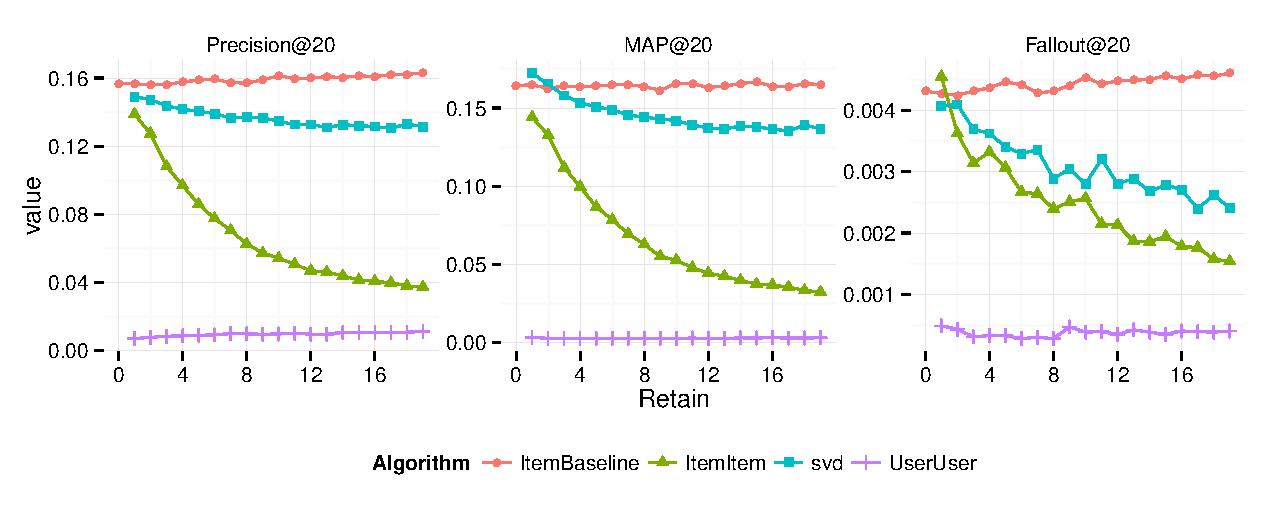
\includegraphics[width=1.1\linewidth]{/export/scratch/kluver/workspace/coldstartrecommendation/lenskit/output/ekstrandTuning/TopNPrecision.pdf}
  \caption{TODO}
  \label{fig:map}
\end{figure*}


  Figure \ref{fig:map} shows MAP@20, precision@20, and fallout@20.
  All three metrics show essentially the same trend, User-User gets the lowest score, the baselines get the highest score.
  On both MAP@20 and precision@20 svd gets a higher score than Item-Item throughout, performing almost as highly as the baseline.
  On fallout@20 Item-Item performs higher than svd and the baseline, but decreases faster than bath, ending with a lower score than either. 
  We also tried recall@20 and mrr@20 and found the same trend.

  This result is rather strange as MAP and precision are metrics where high scores imply better performance, whereas fallout is a metric where high scores imply poor performance.
  This leads to an issue, these metrics contradict each other in terms of the quality of the recommendations from our algorithm.
  One possible reason for this is that these topN metrics are known to be biased toward recommendations that have more popular items \cite{bellogin}.
  Looking at the average popularity (figure \ref{fig:pop}) of recommended items, we see that the average popularity of the recommendations closely replicates the previous three plots.
  Therefore we seek a different, less biased metric to analyze the quality of the recommendations.


  % TopN average rating / topn rmse
    % interpret graph and reason about what it means about quality

\begin{figure*}[ht!]
  \centering
  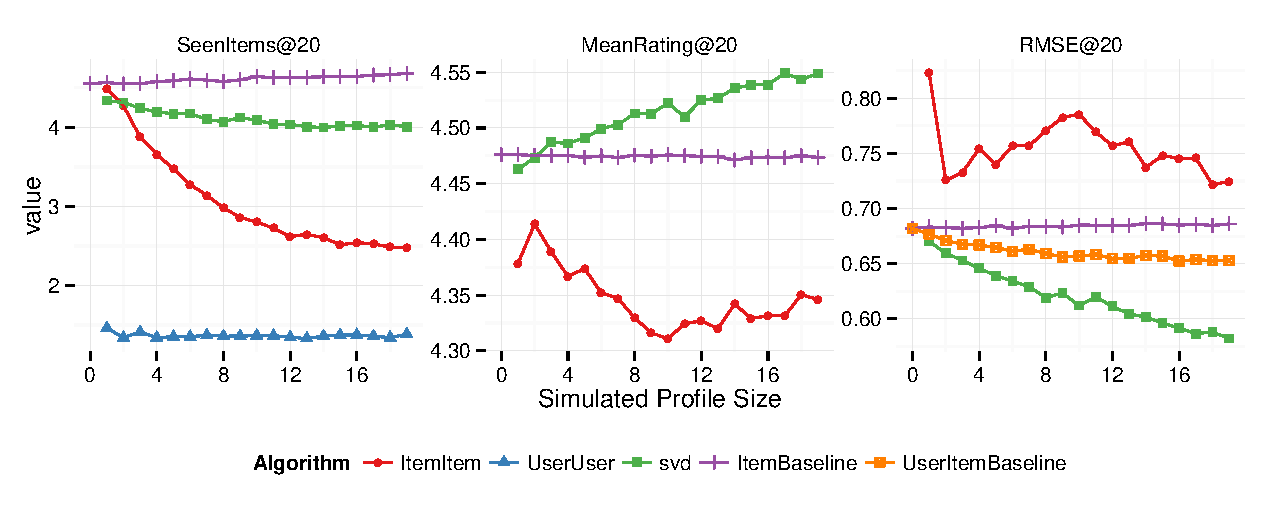
\includegraphics[width=1.1\linewidth]{/export/scratch/kluver/workspace/coldstartrecommendation/lenskit/output/ekstrandTuning/rmse_20.pdf}
  \caption{TODO}
  \label{fig:topN.rmse}
\end{figure*}


  The first graph in figure \ref{fig:topN.rmse} shows the average number of items in the top 20 recommendations for each algorithm that were also in the test set.
  The average number of test set items in recommendations shows a similar trend to the MAP, precision, and recall metrics, user-user getting by far the fewest seen items, and the baseline getting the most.
  %TODO: talk about trust building here!

  The second graph in figure \ref{fig:topN.rmse} shows the average rating for those items in the top 20 recommendations for each algorithm.
  The first thing to note about this graph is that all of these algorithms are doing a reasonable job of recommending items the user might like to watch, with all algorithms averaging above 4 stars (implying that the recommended items are, at least on average, enjoyable).
  SVD performs as expected, starting at close to the same average rating as the baselines, and then slowing improving as more ratings are entered.
  Item-Item performs poorly, not only performing worse than the baseline, but showing worse performance as more ratings are added.
  This is quite possibly a similar trend to the one we observed with RMSE and nDCG, where Item-Item's performance decreased as coverage increased leading to the curved performance at cold start.
  
  During testing with other values of N for this metric and the next, we found that User-User's behavior compared to the other algorithms changed significantly with different values of N.
  This is probably due to the very low rate of having seen items in the recommendations, which makes its value much less stable, than the other algorithms.
  Because of this behavior we will draw no conclusion from User-User's performance on this metric, to avoid accidentally attributing behavior to it, that was instead formed by our choice of 20 as N.
  
  The third graph in figure \ref{fig:topN.rmse} shows the RMSE our algorithms got on items in the top 20 recommendations for each algorithm.
  Not surprisingly, this figure shows the same trends as the last one meaning that the algorithms whose recommendations were (on average) most likable, were those whose recommendations were most accurate.
  Again, SVD performs quite well, Item-Item shows poor performance, and, due to sensitivity of User-User to our choice of N, we make no conclusions about User-User.

\subsection{Other recommender metrics}
  % Other recommender metrics

\begin{figure*}[ht!]
  \centering
  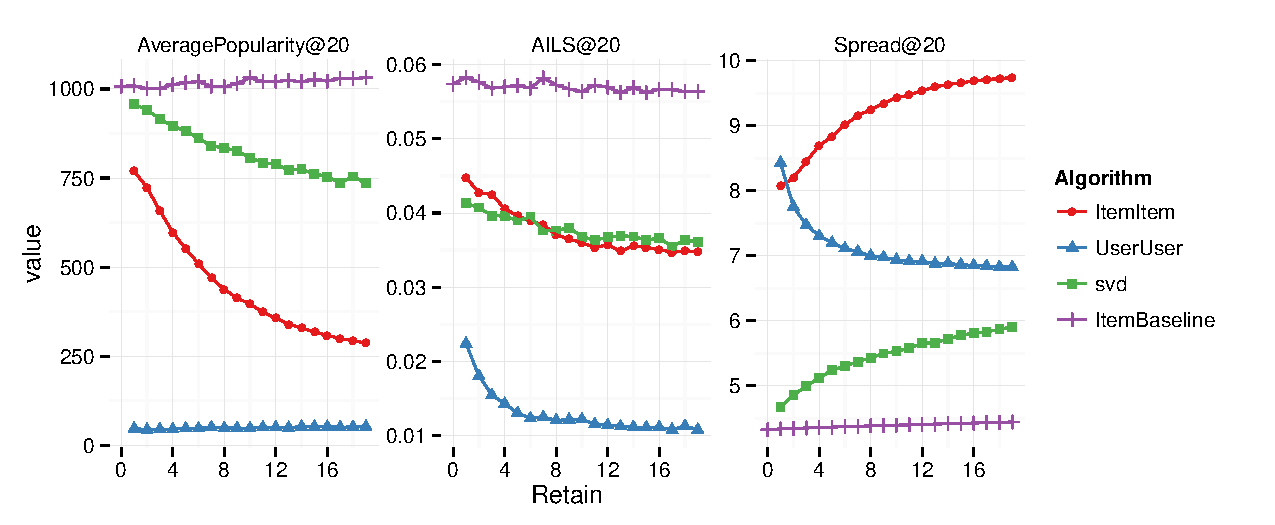
\includegraphics[width=\linewidth]{/export/scratch/kluver/workspace/coldstartrecommendation/lenskit/output/ekstrandTuning/popdiv.pdf}
  \caption{TODO}
  \label{fig:pop}
\end{figure*}


    % popularity graph
  The first graph in figure \ref{fig:pop} shows the average popularity of recommended items by each algorithm.
  %TODO: re-write this
  Across all datapoint sizes the ranking of algorithms is the same, with the baselines recommending the most popular movies, followed by svd, which recommends less popular movies, then Item-Item, which recommends much less popular movies, leaving User-User to recommend the least popular movies.
  Unfortunately, we don't know of any guideline for understanding how popular users desire their recommendations to be.
  That in mind, we expect that users will feel the baseline's popularity (around 1000) is too high, and User-User's popularity (around 50) is too low.
  SVD and Item-Item both seem to perform well, with SVD generating more popular recommendations, than Item-Item, and both algorithms showing a significant trend to make less popular predictions as we know more about the user.

    % diversity plot
  The diversity graph in \ref{fig:pop} shows a similar trend to the popularity trend with the baseline algorithms producing the least diverse list of recommendations and User-User providing by far the most diverse list of recommendations.
  For the first few ratings SVD is able to provide more diverse recommendations than Item-Item.
  However, Item-Item seems to grow in diversity faster than SVD in response to more data, so after 4 ratings Item-Item is providing slightly more diverse recommendations than SVD.
  Overall, Item-Item and SVD are providing recommendations that, at least in an offline context, appear to have quite comparable diversity.


\begin{figure}[ht!]
  \centering
  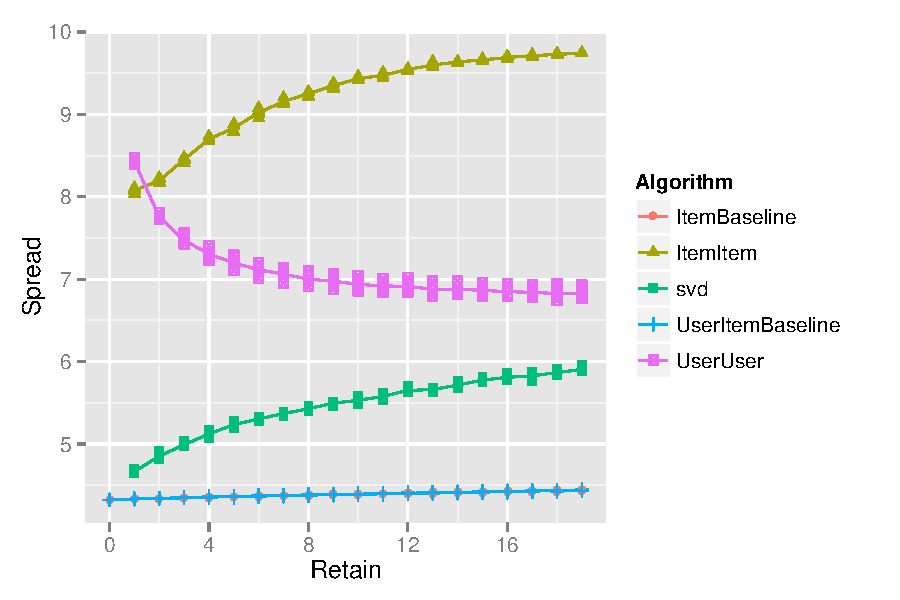
\includegraphics[width=1.1\columnwidth]{/export/scratch/kluver/workspace/coldstartrecommendation/lenskit/output/ekstrandTuning/topN_entropy.pdf}
  \caption{TODO}
  \label{fig:spread}
\end{figure}


  % spread plot
  The graph in \ref{fig:spread} shows the spread of the recommendations from each algorithm.
  Because this metric can only be computed over a group of people, confidence intervals over the per-user average are not provided, instead the specific spread values computed in each five folds are shown as points, with lines connecting the value from the five metrics.
  %TODO: make this point earier and better.
  Like the diversity and popularity metrics we see that the values take a much larger range, with different algorithms seeming to converge to different amounts spread.
  The baseline algorithms, which recommend every user the same list of recommendations (unless the user has rated one of those items) have the lowest spread.
  SVD has the second lowest spread, starting with a spread very close to the baselines and then slowly growing more spread as it gets more ratings.
  Like popularity, we don't know exactly how much spread is best for a recommender system, but we can guess that we want more spread from our recommendations than baseline, and all other things being equal, more spread is probably better.
  Based on this intuition it seems that SVD might have focus on too few items in its recommendations.

  User-User and Item-Item both have significantly more spread than the other algorithms.
  They show interestingly opposite trends, with User-User providing more spread at one rating, and then decreasing, and Item-Item giving less spread and then increasing.
  By 8 ratings, we see that Item-Item has by far the most spread recommendations.
  It is strange that User-User would get less spread as it learns more about users.
  This implies that the more it learns about users, the less spread out its recommendations are.
  This could be some form of a regression towards the mean, where as it learns more about users its recommendations become less personalized to the users individual quirks.
  More research will be needed to understand this trend.
  
\section{Conclusions}
  % summary of results in a big old table.
    % the accuracy of svd and user-user both seemed good. item-item seemed to have trouble especially with very new users.
    % svd did quite well on our traditional topN metrics, item-item did OK, and user-user did bad., but there are flaws with these metrics.
    % on our topN RMSE item-item (again) seemed to have issues, and user-user did quite well, but the low hit rate is troubleing. 
    % again svd seems the winner here.
    % on our fluffy metrics item-item and svd seemed to do well. I might argue that item-item seemed to do better (spread, and higher throughout).
    % user-user seemed to do poor
  % what this means
    % user-user seems to be able to give accurate predictions, but seems to focus on overly obscure items in recommendation.
    % item-item seems to give not-bad recommendations, but its predictions have issues
    % based only on these results svd seems to be the best performer and is our recommendation to new systems.
  % other takeaways
    % regularization
    % if you use a switching recommender, this methodology can help you choose when to switch.
    % non-traditional metrics can tell you more about what is going on, these seem to be more properties of the class of algo than of the data, so its worth looking at these when choosing algorithms, to find one with properties that are good for your task.

  % limitations and opprotunities
    % dataset limitations
      % only one domain
      % no quitters in our dataset
    % metrics limitations
      % many metrics require user data to help us understand what users want from a recommender
      % no well known ``goodness'' metric for topN.
    % algorithm limitations
      % only covered three common families,
      % different algos tuned specifically for cold start.
      % algos that use extra data about users or about items.

  % despite the limitations we were able to show differences between algorithms in a cold start situation.

\section{Acknowledgements}
 TODO:

\bibliographystyle{abbrv}
\bibliography{resources}  % sigproc.bib is the name of the Bibliography in this case

\end{document}
